\documentclass{scrartcl}\usepackage[]{graphicx}\usepackage[]{color}
%% maxwidth is the original width if it is less than linewidth
%% otherwise use linewidth (to make sure the graphics do not exceed the margin)
\makeatletter
\def\maxwidth{ %
  \ifdim\Gin@nat@width>\linewidth
    \linewidth
  \else
    \Gin@nat@width
  \fi
}
\makeatother

\definecolor{fgcolor}{rgb}{0.345, 0.345, 0.345}
\newcommand{\hlnum}[1]{\textcolor[rgb]{0.686,0.059,0.569}{#1}}%
\newcommand{\hlstr}[1]{\textcolor[rgb]{0.192,0.494,0.8}{#1}}%
\newcommand{\hlcom}[1]{\textcolor[rgb]{0.678,0.584,0.686}{\textit{#1}}}%
\newcommand{\hlopt}[1]{\textcolor[rgb]{0,0,0}{#1}}%
\newcommand{\hlstd}[1]{\textcolor[rgb]{0.345,0.345,0.345}{#1}}%
\newcommand{\hlkwa}[1]{\textcolor[rgb]{0.161,0.373,0.58}{\textbf{#1}}}%
\newcommand{\hlkwb}[1]{\textcolor[rgb]{0.69,0.353,0.396}{#1}}%
\newcommand{\hlkwc}[1]{\textcolor[rgb]{0.333,0.667,0.333}{#1}}%
\newcommand{\hlkwd}[1]{\textcolor[rgb]{0.737,0.353,0.396}{\textbf{#1}}}%

\usepackage{framed}
\makeatletter
\newenvironment{kframe}{%
 \def\at@end@of@kframe{}%
 \ifinner\ifhmode%
  \def\at@end@of@kframe{\end{minipage}}%
  \begin{minipage}{\columnwidth}%
 \fi\fi%
 \def\FrameCommand##1{\hskip\@totalleftmargin \hskip-\fboxsep
 \colorbox{shadecolor}{##1}\hskip-\fboxsep
     % There is no \\@totalrightmargin, so:
     \hskip-\linewidth \hskip-\@totalleftmargin \hskip\columnwidth}%
 \MakeFramed {\advance\hsize-\width
   \@totalleftmargin\z@ \linewidth\hsize
   \@setminipage}}%
 {\par\unskip\endMakeFramed%
 \at@end@of@kframe}
\makeatother

\definecolor{shadecolor}{rgb}{.97, .97, .97}
\definecolor{messagecolor}{rgb}{0, 0, 0}
\definecolor{warningcolor}{rgb}{1, 0, 1}
\definecolor{errorcolor}{rgb}{1, 0, 0}
\newenvironment{knitrout}{}{} % an empty environment to be redefined in TeX

\usepackage{alltt}

\usepackage[utf8]{inputenc}
\usepackage{graphicx}%GRaphiken
\usepackage{tabularx}%Tabellen!
\usepackage[english]{babel}% Zeilentrennung besser
\usepackage{url}% Urls besser
\usepackage{textcomp}% Sonderzeichen
\usepackage{amsmath}%maths / equations
\usepackage{helvet}% Schrift Helvetica
% \usepackage[helvet]{sfmath}% Helvet also in Math modes
% \renewcommand\familydefault{\sfdefault}
\usepackage{sansmath} % sans in math
\usepackage{todonotes}
\usepackage[
	left=3cm,
	right=2cm,
	top=1.5cm,
	bottom=1cm
	,
	includeheadfoot
	]{geometry}														% Satzspiegel
\usepackage[
	round,	%(defaultage in the main file and \input ) for round parentheses;
	%square,	% for square brackets;
	%curly,	% for curly braces;
	%angle,	% for angle brackets;
	colon,	% (default) to separate multiple citations with colons;
	%comma,	% to use commas as separaters;
	authoryear,% (default) for author-year citations;
	%numbers,	% for numerical citations;
	%super,	% for superscripted numerical citations, as in Nature;
	sort,		% orders multiple citations into the sequence in which they appear in the list of 				references;
	%sort&compress,    % as sort but in addition multiple numerical citations
                   % are compressed if possible (as 3-6, 15);
	%longnamesfirst,  % makes the first citation of any reference the equivalent of
                   % the starred variant (full author list) and subsequent citations
                   %normal (abbreviated list);
	%sectionbib,      % redefines \thebibliography to issue \section* instead of \chapter*;
                   % valid only for classes with a \chapter command;
                   % to be used with the chapterbib package;
	%nonamebreak,     % keeps all the authors names in a citation on one line;
                   %causes overfull hboxes but helps with some hyperref problems.
]{natbib}											    			% Literaturverzeichnis
\usepackage{scrhack}   % kills \float@addtolists!  warning
\usepackage[pdfpagelabels,plainpages=false, pageanchor=false]{hyperref}	


%% andere Einstellungen
\linespread{1.5}% 1.5 Zeilenabstand			
\graphicspath{{fig/}}                     % path to graphics

\title{Use the GLM, Luke!}
\subtitle{How the use of proper statistical models can increase statistical power in ecotoxicological experiments.}
\author{Eduard Szöcs}
\date{\today}
\IfFileExists{upquote.sty}{\usepackage{upquote}}{}
\begin{document}
\maketitle

\section{Introduction}

In environmental risk assessments statistical tests play an important role to evalute the effects of pesticides, e.g. in finding the Lowest Observed Effect Concentration (LOEC).
Ecotoxicologists perform various kinds of experiments yielding to different types of data.
Examples are: animal counts in mesocosm experiments (positive and discrete data), 
proportions of surviving animals (bonded between 0 and 1) or biomass (positive data).

These types of data are inherently not normally distributed. 
However, in order to use the more familiar and traditional data analysis methods based on normal distribution, ecotoxicologists try to transform their data to met these assumptions. 
Survivals with binomial distributed data (x out ouf n) are usually transformed using a arcsin square root transformation \citep{oecd_current_2006,
newman_quantitative_2012},
count data using a log(Ax + 1) transformation \citep{van_den_brink_impact_2000}.
If the transformed data does not met the normality assumptions, non-parametric tests are usually applied \citep{wang_making_2011}.

However, there is also a third possibility:
Using a distribution fitting to the type of data instead of the normal distribution, namely \emph{Generalized Linear Models} (GLM) \citep{nelder_generalized_1972}. 
GLMs can handle various types of data distributions, e.g. poisson or negative binomial (counts), binomial (proportions) or gamma (mass); the normal distribution being a special case.
Despite that GLMs were available more than 40 years now, ecotoxicologist do not make use of them.
One reason might be that they are not mentioned in standard guidance documents for statistical analysis of ecotoxilogical experiments:
GLMs are not discussed in the \citep{oecd_current_2006} and \citep{epa_methods_2002} guidelines and are not included in the respective schemes for hypothesis testing. 
\citet{newman_quantitative_2012} does not cover GLMs in his book.
\citet{environment_canada_guidance_2005} term GLMS as \emph{useful for toxicological research}, but did not include them in their schemes as \emph{the concept is quite advanced and as yet is not widely used in environmental toxicology}.

Recently studies concluded that data transformations should be avoided and GLMs be used as they have better statistical properties (\emph{Do not log-transform count data}, \citep{ohara_not_2010}; \emph{The arcsine is asinine}, \citep{warton_arcsine_2011}).
In this paper we first review what types of analysis are used by ecotoxicologists.
Then we demonstrate that GLM provide superior properties compared to data transformation. 
We used simulated data that mimicked data encountered in ecotoxicology to compare GLMs with two common data types: counts and proportions. 
Methods were compared in terms of Type I error (maintain a significance level of 0.05 when there is no effect) and power (detect an effect when it is present). 



\section{Methods}
\subsection{Review}
Literature review of SETAC Journals -> NOEC, GLM, log/arcsine transformation? How often, what is applied?

\subsection{Simulations}
\subsubsection{Count data}
We simulated count data that mimics count data encountered in mesocosm experiments, with five treatments (T1 - T5) and one control group (C) (e.g. \citep{brock_minimum_2014}).
Counts were drawn from a negative binomial distribution with a fixed dispersion parameter for all treatments ($\theta = 3.91$).
We simulated datasets with different the number of replicates (N = \{3, 6, 9, 12\}) and different abundances in control treatments ($\mu_\text{\tiny C}$ = \{2, 4, 8, 16, 32, 128, 512, \}). 
For each combination we generated 100 datasets.
For power estimation mean abundance in treatments T2 - T5 was reduced to half of the control treatment and T1 ($\mu_\text{\tiny T2} = ... = \mu_\text{\tiny T5} = 0.5 \mu_\text{\tiny C} = 0.5 \mu_\text{\tiny T1} $).
For Type I error estimation mean abundance was equal between all groups.

We fitted two parametric models to this data.
First a model assuming a normal distribution after a ln(Ay + 1) transformation the response (eqn \ref{eqn:1}).

\begin{align}
  y^T_i = log(Ay_i + 1) \\
  y^T_i \sim N(\mu_i, \sigma^2) \nonumber \\
  y^T_i = \alpha + \beta x_i \label{eqn:1} \\
  var(y^T_i) = \sigma^2 \nonumber
\end{align}
where y is the measured abundance and A was selected in such a way that the lowest non-zero abundance of the data set is transformed to 1 \citep{van_den_brink_impact_2000}. 
$y^T$ is the transformed abundance and the model assumes a constant variance.

And second GLM assuming that the response follows a negative binomial distribution with a log-link (eqn \ref{eqn:2}) and
the variance is a quadratic function of the mean.

\begin{align}
  y_i \sim NB(\mu_i, \theta)  \nonumber \\
  log(\mu_i) = \alpha + \beta x_i   \label{eqn:2} \\
  var(y_i) = \mu_i + \mu_i^2 / \theta  \nonumber
\end{align}

Additionally we also analysed this data using a non-parametric approach (see below).

\subsubsection{Binomial data}
We simulated binomial data that mimics data encountered in survival experiments, with five treatments (T1 - T5) and one control group (C) (e.g. \citep{newman_quantitative_2012}, example 5.1 therein).
Each group consisted of 10 animals and was sampled from a Bin(10, p) distribution.
For power simulation p in the control and T1 was held constant at p = 0.9 and varied for T2 - T5  (p = \{0.5, 0.55, 0.60, ... , 0.90\}).
For Type I error simulations p was equal between groups ($p_c = p_{T1} = ... = p_{T6}$; p = \{0.5, 0.55, 0.60, ... 0.90\}).
In both simulations we also varied the number of replicates (N = \{3, 6, 9, 12\}).
For each combination we generated 100 datasets.

We fitted two parametric models to this data.
First a model assuming a normal distribution after arcsin transforming the response (eqn \ref{eqn:3} + \ref{eqn:4}, \citep{epa_methods_2002}).
\todo{original reference Bartlett 1937!}

\begin{align}
  y^T_i = 
  \begin{cases}
    arcsin \sqrt{1/4n}, & \text{if } y_i = 0 \\
    arcsin(1) - arcsin \sqrt{1/4n}, & \text{if } y_i = 1 \\
    arcsin \sqrt{y / n}, & otherwise
  \end{cases}
  \label{eqn:3}
\end{align}

where y are the number of dead animals, $y^T$ are the transformed proportions and n is the number of animals per replicate (n = 10).

\begin{align}
  y^T_i \sim N(\mu_i, \sigma^2) \nonumber \\
  y^T_i = \alpha + \beta x_i \label{eqn:4} \\
  var(y^T_i) = \sigma^2 \nonumber
\end{align}

And second a model assuming a binomial distribution of the response with a logit link (eqn \ref{eqn:5}).

\begin{align}
  y_i \sim Bin(\pi_i, 10) \nonumber \\
  logit(\pi_i) = \alpha + \beta x_i \label{eqn:5} \\
  var(y_i) = 10 \times \pi_i \times (1 - \pi_i) \nonumber
\end{align}

where y is the number of dead animals (out of ten) and $\pi$ the probabilty of encountering a dead animal.

\subsubsection{Comparing methods}
A global treatment effect was investigated using Likelihood-Ratio-Tests.
Moreover, we applied a non-parametric Kruskal-Wallis-Rank-Sum-Test on the untransformed data.

We also investigated power and Type I error for detecting the LOEC (T1 in the simulations).
For the parametric models we used the parametrisation of contrasting to the control group (equivalent to Dunnett contrast).
\todo{Wald!-test}
We used a pairwise Wilcoxon-Rank-Sum-Test as a anon-parametric method to detect the LOEC.
P-values were adjusted for multiple tesing using Holm's procedure.

All simulations have be done in R (Version 3.1.1) on a 64-bit Linux machine with 8 GB and 2.2 GHz.
Exemplary analysis of real data (Count data \citep{brock_minimum_2014}, survial data \citep{epa_methods_2002}) can be found in the supplement.
Source code for this work is available online at \url{https://github.com/EDiLD/usetheglm}. 


\section{Results}
\subsection{Review}

\subsection{Simulations}
\begin{figure}
  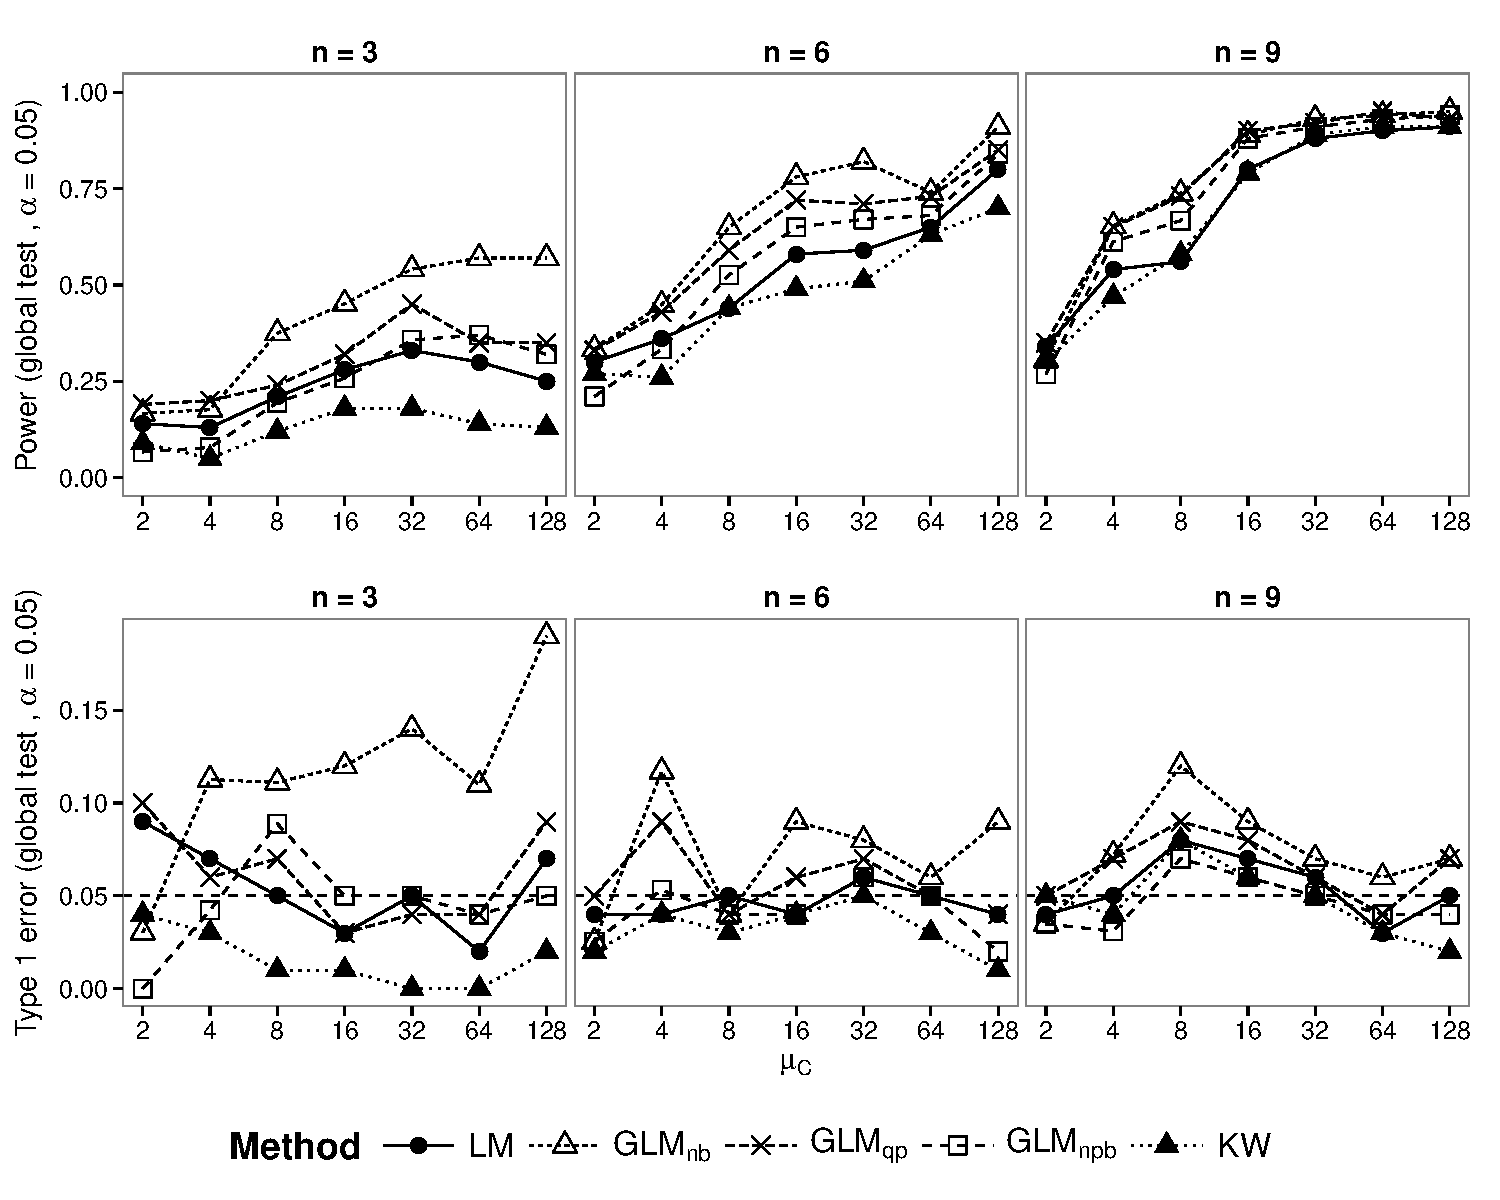
\includegraphics[width=\linewidth]{p_glob_c.pdf}
  \caption{Simulation results from power (upper) and Type I error simulations (lower) for count data.}
  \label{fig:p_glob_c}
\end{figure}
\todo{Check legend -> wilcox is not correct!}

\begin{figure}
  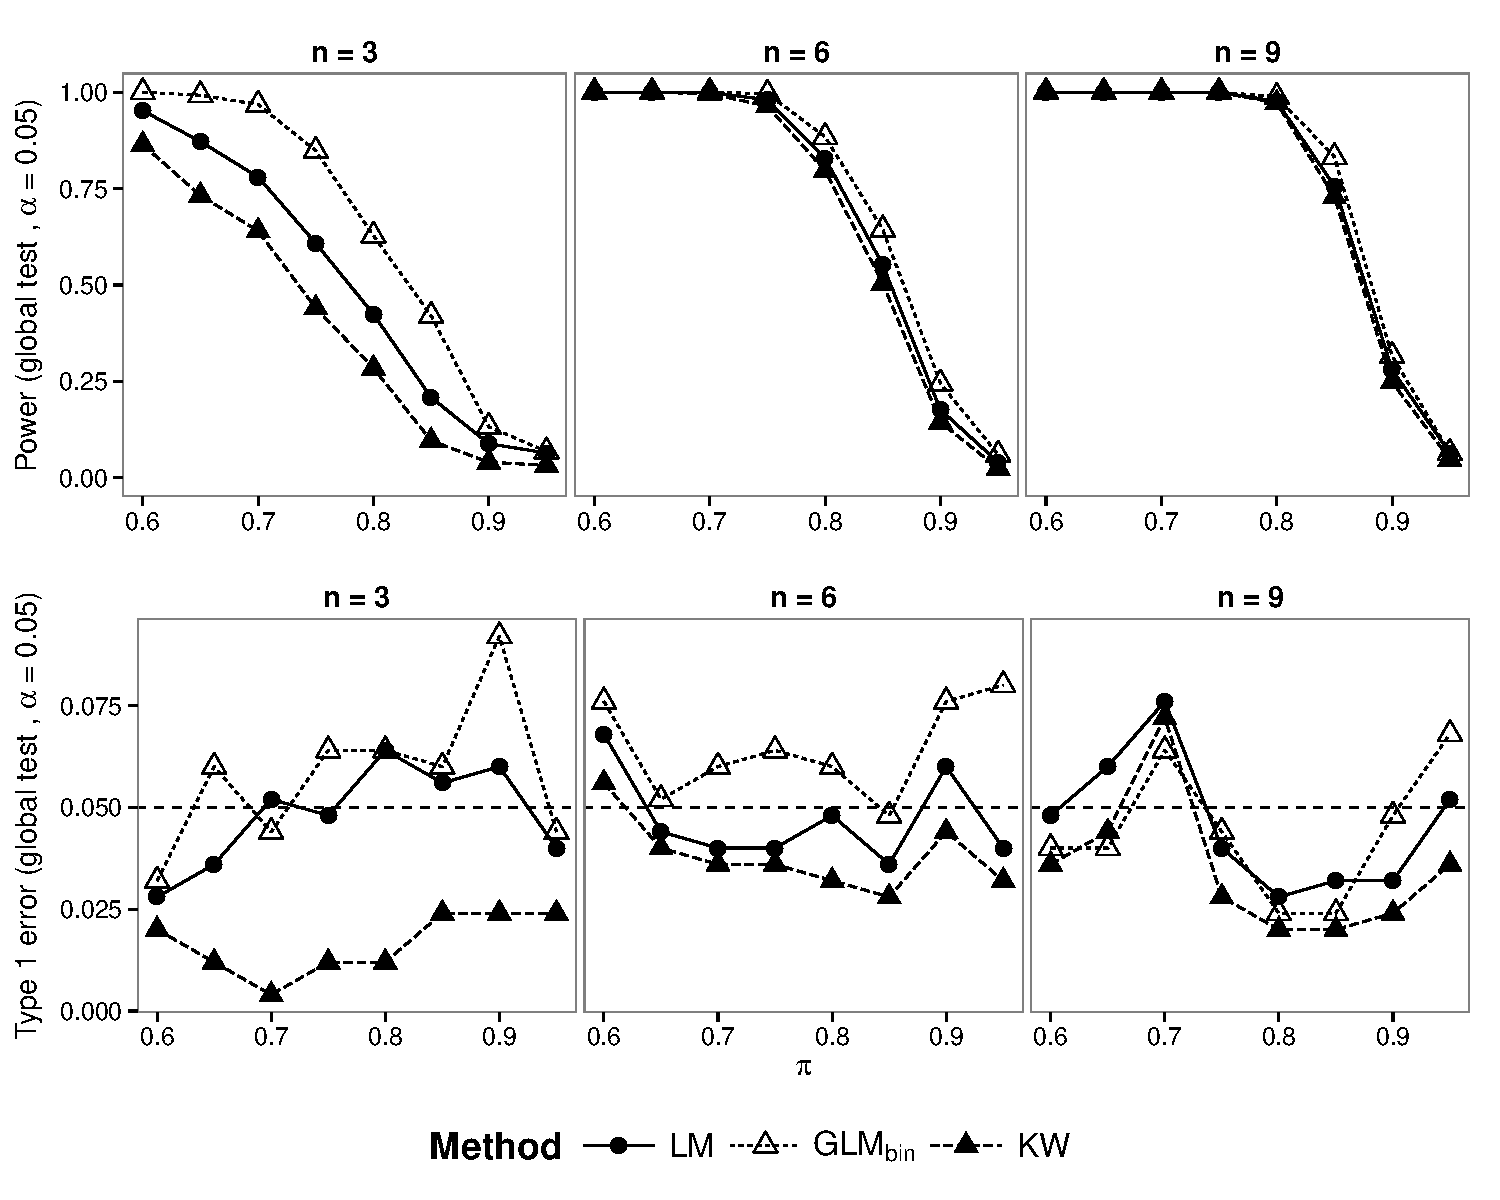
\includegraphics[width=\linewidth]{p_glob_p.pdf}
  \caption{Simulation results from power (upper) and Type I error simulations (lower) for binomial data.}
\end{figure}

\todo{Double Check results! Line by Line!}
\todo{Why did we find increased Type I error and Warton did not? Maybe a different asin? (we use a special form, warton standard)}



\section{Discussion}


\section{Conclusion}

\todo{advise, supplement, shapiro scheisse, sessionInfo to Supplement}

\bibliography{references}
\bibliographystyle{apalike}

\end{document}
